
\documentclass[article]{beamer}
\usepackage{beamerthemesplit,fancybox,verbatim, wasysym}
\usepackage{graphicx,pgfarrows,pgfnodes, tikz, tabu, mathrsfs}
\usepackage[utf8]{inputenc} 
\usepackage[T1]{fontenc}
\newtheorem{thm}{Theorem}
\theoremstyle{definition}
\newtheorem*{ex}{Example}
\newtheorem{cor}{Corollary}[section]
\newtheorem{lem}[thm]{Lemma}
\newtheorem{conjecture}[thm]{Conjecture}
\newtheorem{prop1}[thm]{Proposition 1}
\newtheorem{prop2}[thm]{Proposition 2}
\newtheorem{prop3}[thm]{Proposition 3}
\newtheorem{prop4}[thm]{Proposition 4}
\newtheorem{prop5}[thm]{Proposition 5}
\newtheorem{prop6}[thm]{Proposition 6}
\newtheorem{prop7}[thm]{Proposition 7}
\newtheorem{proposition}[thm]{Proposition}
\newtheorem{wild_spec}[thm]{Wild Speculation}
\theoremstyle{remark}
\newtheorem*{rem}{Remark}
\theoremstyle{definition}
\newtheorem{defn}{Definition}[section]
\theoremstyle{definition}
\newtheorem*{ack}{Acknowledgements}
\def\Q{\mathbb{Q}}
\def\F{\mathbb{F}}
\def\Gal{{\rm Gal}}
\def\Cl{{\rm Cl}}
\newcommand{\legen}[2]{\genfrac{(}{)}{}{}{#1}{#2}}
\def\ord{{\rm ord}}
\def\Tr{{\rm Tr}}
\def\d{d}
\def\const{\text{const}}
\newcommand{\leg}[2]{\genfrac{(}{)}{}{}{#1}{#2}}
\newcommand{\noframe}[1]{}

\newcommand{\bfrac}[2]{\genfrac{}{}{}{0}{#1}{#2}}
\newcommand{\sm}[4]{\left(\begin{smallmatrix}#1&#2\\ #3&#4 \end{smallmatrix} \right)}
\newcommand{\mfG}{\mathfrak{G}}
\newcommand{\mfF}{\mathfrak{F}}
\newcommand{\pr}{\text {\rm pr}}
\newcommand{\calM}{\mathcal{M}}
\newcommand{\calW}{\mathcal{W}}
\newcommand{\calC}{\mathcal{C}}
\newcommand{\calP}{\mathcal{P}}
\newcommand{\calq}{\mathcal{q}}
\newcommand{\mfq}{\mathfrak{q}}
\newcommand{\mfp}{\mathfrak{p}}
\newcommand{\mfa}{\mathfrak{a}}
\newcommand{\mfc}{\mathfrak{c}}
\newcommand{\mfm}{\mathfrak{m}}
\newcommand{\Fqt}{\mathbb{F}_q[t]}
\newcommand{\calO}{\mathcal{O}}
\newcommand{\calA}{\mathcal{A}}
\newcommand{\calN}{\mathcal{N}}
\DeclareMathSymbol{\mlq}{\mathord}{operators}{``}
\DeclareMathSymbol{\mrq}{\mathord}{operators}{`'}
\newcommand{\GG}{\mathcal{G}}
\newcommand{\calS}{\mathcal{S}}
\newcommand{\calR}{\mathcal{R}}
\newcommand{\FF}{\mathcal{F}}
\newcommand{\QQ}{\mathcal{Q}}
\newcommand{\cO}{\mathcal{O}}
\newcommand{\Mp}{\text {\rm Mp}}
\newcommand{\mathfrakG}{\mathfrak{G}}
\newcommand{\Qmd}{\mathcal{Q}_{m,d}}
\newcommand{\la}{\lambda}
\newcommand{\R}{\mathbb{R}}
\newcommand{\C}{\mathbb{C}}
\newcommand{\Qd}{\mathcal{Q}_d}
\newcommand{\Z}{\mathbb{Z}}
\newcommand{\N}{\mathbb{N}}
\newcommand{\SL}{{\text {\rm SL}}}
\newcommand{\GL}{{\text {\rm GL}}}
\newcommand{\GO}{{\text {\rm GO}}}
\newcommand{\add}{{\text {\rm add}}}
\newcommand{\sub}{{\text {\rm sub}}}
\newcommand{\Aut}{{\text {\rm Aut}}}
\newcommand{\Sym}{{\text {\rm Sym}}}
\newcommand{\Disc}{{\text {\rm Disc}}}
\newcommand{\sgn}{\operatorname{sgn}}
\newcommand{\PSL}{{\text {\rm PSL}}}
\newcommand{\Stab}{\textnormal{Stab}}
\newcommand{\Op}{\mathcal{O}_K}
\newcommand{\h}{\mathfrak{h}}
\newcommand{\G}{\Gamma}
\newcommand{\g}{\gamma}
\newcommand{\zaz}{\Z / a\Z}
\newcommand{\znz}{\Z / n\Z}
\newcommand{\ve}{\varepsilon}
\newcommand{\tr}{{\text {\rm tr}}}
\newcommand{\odd}{{\text {\rm odd}}}
\newcommand{\bk}{B_k}
\newcommand{\rr}{R_r}
\newcommand{\rk}{{\text {\rm rk}}}
\newcommand{\Tor}{{\text {\rm Tor}}}
\newcommand{\disc}{\textnormal{disc}}
\newcommand{\textmod}{\textnormal{mod}}
\newcommand{\sump}{\sideset{}{'}\sum}
\newcommand{\gkr}{\mathfrak{g}_{k,r}}
\newcommand{\re}{\textnormal{Re}}
\newcommand{\Res}{\textnormal{Res}}
\newcommand{\im}{\textnormal{Im}}
\newcommand{\orange}[1]{{\leavevmode\color{orange}{#1}}}
\newcommand{\blue}[1]{{\leavevmode\color{blue}{#1}}}
\newcommand{\purple}[1]{{\leavevmode\color{purple}{#1}}}
\newcommand{\green}[1]{{\leavevmode\color{green}{#1}}}
\newcommand{\olive}[1]{{\leavevmode\color{olive}{#1}}}

\newcommand{\red}[1]{{\leavevmode\color{red}{#1}}}
\newcommand{\white}[1]{{\leavevmode\color{white}{#1}}}


\definecolor{Dblue}{rgb}{.255,.41,.884}
\definecolor{Gorange}{rgb}{.196,.804,.466}

\author[Frank Thorne]{Frank Thorne}
\title[Number Field Counting]{An Overview of Number Field Counting}
\date{Qu\'ebec-Vermont Number Theory Seminar}
\institute{University of South Carolina}
\begin{document}

\frame{\titlepage}

\frame{ \frametitle{Number Field Counting}

\begin{definition}
For any integer $d \geq 1$, write
\[
N_d(X) := \# \{ K \ : \ [K : \Q] = d, \ |\Disc(K)| < X\}.
\]
\onslide<2->
and for each transitive subgroup $G \subseteq S_d$,
\[
N_d(X, G) := \# \{ K \ : \ [K : \Q] = d, \ |\Disc(K)| < X, \ \Gal(K^c/\Q) = G \},
\]
\onslide<3->
so that
\[
N_d(X) = \sum_{\substack{G \subseteq S_d \\ \textnormal{transitive}}} N_d(X, G).
\]
\end{definition}
\onslide<4->
% Comment about more general extensions
}

\frame{ \frametitle{Basic Results}

\begin{theorem}[Finiteness -- Hermite]
For each $d$ and $X$, $N_d(X)$ is finite.
\end{theorem}

\onslide<2->
\begin{theorem}[Minkowski's Lower Bound]
If $[K : \Q] = d$, then
\[
|\Disc(K)| \geq \left( \frac{d^d}{d!} \right)^2 \left( \frac{\pi}{4} \right)^d.
\]
\onslide<3->
In other words,
\[
N_d(X) = 0 \ \textnormal{ for } \ X < (5.803\dots + o(1))^d.
\]
\end{theorem}
}

\frame{ \frametitle{The Inverse Galois Problem}

\begin{conjecture}
For every $d$ and transitive subgroup $G \subseteq S_d$,
\[
X \textnormal{ big enough } \Longrightarrow N_d(X, G) \neq 0.
\]
\end{conjecture}

\vskip 0.1in
\onslide<2->
\begin{proof} 

\begin{center} {\bf \red{(Your Name Here)} }
\end{center}
\end{proof}
}

\frame{ \frametitle{Malle's Conjecture}

\begin{conjecture}
In fact we have
\[
N_d(X, G) \sim c(G) X^{1/a(G)} (\log X)^{b(G)},
\]
where $a(G) \geq 1$ and $b(G) \geq 0$ are \blue{explicitly described} integers.
\end{conjecture}

\vskip 1in
\onslide<2->
%blah blah

}

\frame{ \frametitle{Four Methods to Count Number Fields}

\begin{itemize}
\item<1->
\blue{Generator methods} \olive{(Schmidt, Ellenberg-Venkatesh, ...)}

\onslide<2->
Count in terms of appropriate \orange{algebraic integers}.

\onslide<3->
\purple{Usually seeking upper bounds}.
\item<4->
\blue{Abelian methods} \olive{(Cohn, Wright, M\"aki, ...)}

\onslide<5->
Use \orange{class field theory} and/or \orange{Kummer theory}.

\onslide<6->
\purple{Get good results when $G$ is abelian.}

\item<7->
\blue{Parametrization methods} \olive{(Davenport-Heilbronn, Bhargava, ...)}

\onslide<8->
Count \orange{lattice points} in \orange{prehomogeneous representations}.

\onslide<9->
\purple{Brilliant when it works.}

\item<10->
\blue{Inductive methods} \olive{(Kl\"uners, Cohen-Diaz-Olivier, ...)}

\onslide<11->
Obtain \orange{old results from new}.

\onslide<12->
\purple{Expand the scope of existing methods.}

\end{itemize}
}

\frame{ \frametitle{Generator methods}

If $\alpha \in \mathcal{O}_K$ is a generator of $K/\Q$, then $\Z[\alpha] \subseteq \mathcal{O}_K$ and
\begin{align*}
 |\Disc(\mathcal{O}_K)| = \ & \Disc(\Z[\alpha]) \cdot [\mathcal{O}_K : \Z[\alpha]]^{-2} \\
 = \ & \Disc(\textnormal{minpoly}_{\alpha}) \cdot [\mathcal{O}_K : \Z[\alpha]]^{-2}.
\end{align*}
\onslide<2->
\begin{theorem}[Schmidt]
For each $d$ we have
\[
N_d(X) \ll X^{\frac{d + 2}{4}}.
\]
\end{theorem}
}

\frame{ \frametitle{Schmidt's proof}
\begin{itemize}
\item<2->By \blue{Minkowski's theory}, there exists $\alpha \in \mathcal{O}_K$ with \purple{trace $0$}
and \purple{$||\alpha||_{\sigma} \ll |\Disc(K)|^{\frac{1}{2n - 2}}$} for all embeddings $\sigma : K \mapsto \C$.
\item<3->\blue{Assume that $\Q(\alpha) = K$.} \olive{(If not, induct.)}
\item<4->The \blue{minimal polynomial of $\alpha$} is
\[
\textnormal{minpoly}_{\alpha}(x) = \prod_{\sigma} (x - \sigma(\alpha)) = 
x^n + a_2(\alpha) x^{n - 2} + \cdots + a_n(\alpha),
\]
\vskip -0.17in
\[
\textnormal{with} \ \ \ \purple{a_i(\alpha) \in \Z, \ \ |a_i(\alpha)| \ll |\Disc(K)|^{\frac{i}{2n - 2}}}.
\]
\item<5->
There are at most \blue{$O(X^{\frac{d + 2}{4}})$} possibilities.
\end{itemize}
\onslide<6->
% how can we improve this ... ? 
}

\frame{ \frametitle{Abelian methods}

Given a base number field $K$.
\onslide<2->
\begin{theorem}[Class Field Theory]
Abelian extensions $L/K$ of degree $d$ and {\itshape conductor} dividing 
$\mathfrak{m}$ are in bijection with index $d$ quotients of $\Cl_{\mathfrak{m}}(L)$.
\end{theorem}
\onslide<3->
\begin{theorem}[Kummer Theory]
If in addition $\mu_d \subseteq K$, then abelian extensions $L/K$ of exponent $d$
are in bijection with subgroups of $K^{\times} / (K^{\times})^d$.
\end{theorem}
}

\frame{ \frametitle{Cyclic cubic fields}

\begin{theorem}[Cohn, 1954] We have
\[
\sum_{K \ \textnormal{cyclic cubic}} \frac{1}{\Disc(K)^s} = - \frac{1}{2} + \frac{1}{2} \bigg( 1 + \frac{1}{3^{4s}} \bigg) \prod_{p \equiv 1 \pmod 6}
\bigg(1 + \frac{2}{p^{2s}}\bigg)\;.
\]
\end{theorem}

\begin{corollary}
We have
\[
N_3(X, C_3) \sim \frac{11 \sqrt{3}}{36 \pi} \prod_{p \equiv 1 \pmod{6}}
\frac{(p + 2) (p - 1)}{p (p + 1)}.
\]
\end{corollary}

}

\frame{ \frametitle{General abelian number fields}

\begin{theorem}[Wright, M\"aki, \orange{but read Wood's treatment}]
Let $G$ be any abelian group of order $n$. Then we have
\[
\sum_{\Gal(K/\Q) \simeq G} \frac{1}{\Disc(K)^s} = \textnormal{ \purple{finite sum of Euler products} }.
\]
\end{theorem}

\begin{corollary} We have
\[
N_{|G|}(X, G) \sim c(G) X^{1/a(G)} (\log X)^{b(G)},
\]
where $a(G)$ and $b(G)$ are explicit and $c(G)$ is `explicit'.
\end{corollary}
}

\frame{ \frametitle{Prime degree (Cohen, Diaz y Diaz, Olivier 2002)}

\footnotesize{\itshape{``It is claimed that this constant can be explicitly computed as a a finite product of local adelic integrals,
but in practice this has not been done, even for the simplest Abelian groups $G$, except for $G = C_2$...''}}
\onslide<2->
\begin{center}
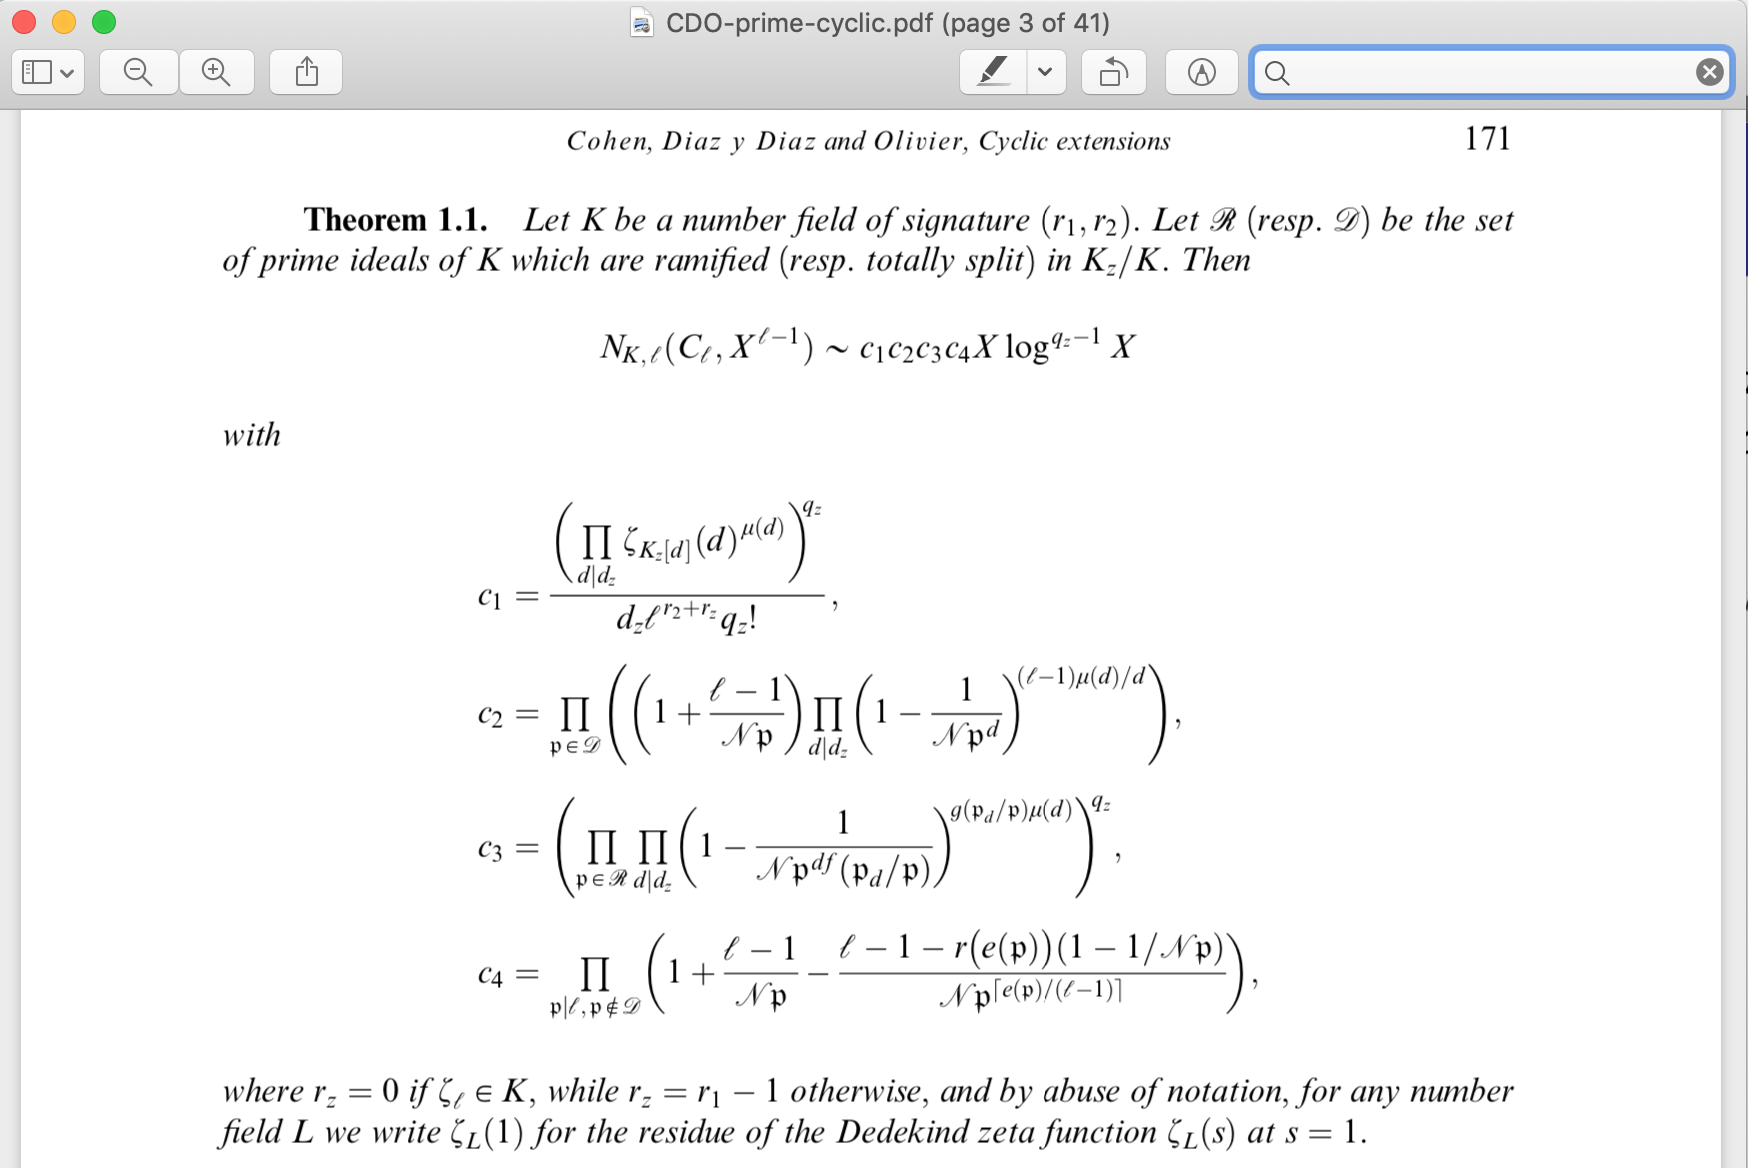
\includegraphics[width=0.81\textwidth]{cdo-theorem-2.png}
\end{center}
}

%\frame{ \frametitle{Sample theorem}
%
%\begin{definition}
%If $K$ is an $S_3$- cubic field, its {\itshape quadratic resolvent} is $\Q(\sqrt{\Disc(K)})$,
%the unique quadratic subfield of $K^c$.
%\end{definition}
%
%\begin{theorem}[Cohen, Morra, T.]
%Let $D \neq 0, 1$ be a fundamental discriminant. Then,
%\[
%\sum_{\substack{[K : \Q] = 3 \\ \Q(\sqrt{D}) \textnormal{ is the} \\ \textnormal{quadratic resolvent of $K$}}} |\Disc(K)| = 
%\{ \textnormal{explicit finite sum of Euler products} \}.
%\]
%\end{theorem}
%
%
%}

\frame{ \frametitle{The parametrization method}
\begin{center}
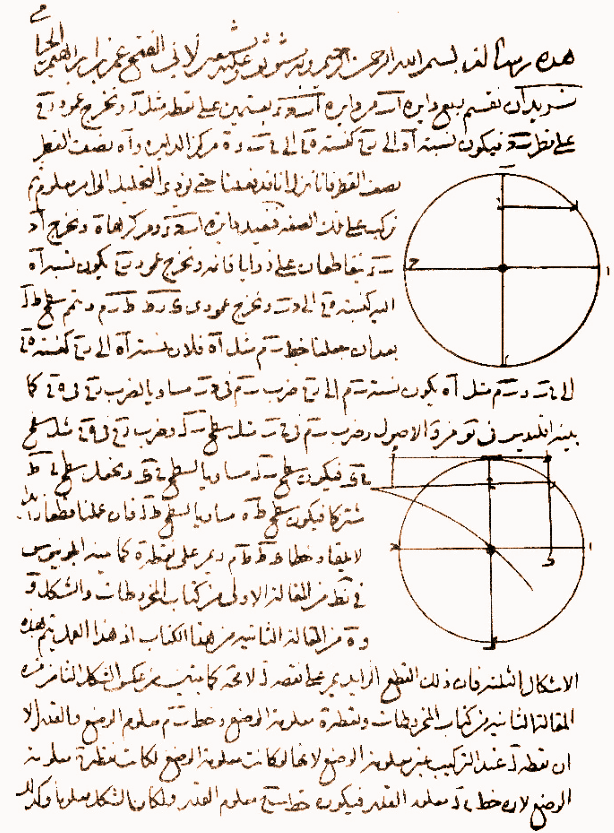
\includegraphics[width=0.5\textwidth]{khayyam.png}
\end{center}
}

\frame{ \frametitle{Intersections of conics}
Example. \blue{Solve $x^4 - x^3 + 3x^2 - 5x + 1 = 0$.}

\onslide<2->
\[
\orange{y} = \blue{x^2}, \ \ \orange{y^2} - \blue{y} \orange{x} + 3\orange{y} - 5\blue{x} + 1 = 0.
\]
\onslide<3->
\begin{center}
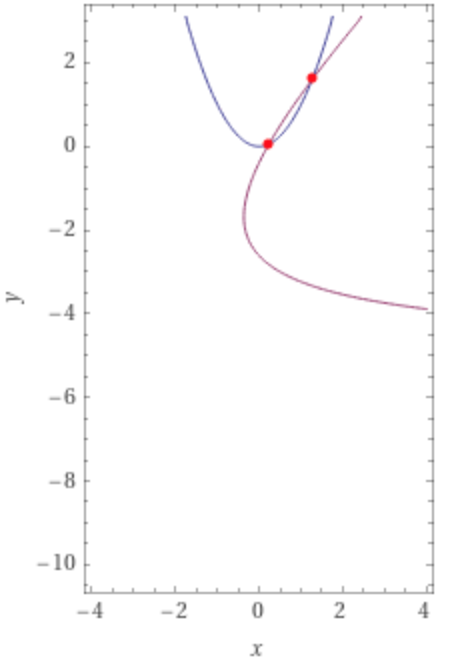
\includegraphics[width=0.36\textwidth]{conics2.png}
\end{center}
}

\frame{ \frametitle{A sample theorem}

\begin{theorem}[Bhargava, {\itshape Annals}, 2004]
There exists an {\itshape explicit, discriminant preserving} bijection between the following
two sets:
\begin{itemize}
\item<2->
$\GL_3(\Z) \times \GL_2(\Z)$-orbits on the lattice
$(\Sym^2 \Z^3 \otimes \Z^2)$ of {\bf pairs of integral ternary quartic forms}.
\item<3->
Pairs $(Q, R)$, where $Q$ is a {\bf quartic ring} and $R$ is a {\bf cubic resolvent} of $Q$.
\end{itemize}
\end{theorem}
}

\frame{ \frametitle{A Bhargava-style metatheorem}

\begin{theorem}
There exists an explicit, discriminant preserving bijection between the following two sets:
\begin{itemize}
\item<2->
$G(\Z)$-orbits on a lattice $V(\Z)$; where $G$ is an {\bf algebraic group} acting
(often {\bf prehomogeneously}) on a vector space $V$;
\item<3->
Some nice class of arithmetic objects we want to count.
\end{itemize}
\end{theorem}

}

\frame{ \frametitle{How to prove Bhargava-style theorems}

\begin{itemize}
\item<2->
Read old papers in representation theory, invariant theory, and commutative algebra for inspiration. \onslide<3-> (\blue{Or Omar Khayyam!})
\item<4->
Pick your favorite complex representation $(G, V)$ (\blue{which should be defined over $\Z$, and for which the invariant
theory should be nice}).
\item<5->
Try to prove that the $G(\Z)$-orbits on $V(\Z)$ parametrize something. \onslide<4-> \blue{Hope to get lucky}.
\end{itemize}
}

\frame{ \frametitle{Counting Low Degree Fields }

\begin{theorem}[Davenport-Heilbronn, Bhargava, et al.]
We have
\[
N_3 (X) = \frac{1}{3 \zeta(3)} X + 
\frac{4 (1 + \sqrt{3}) \zeta(1/3)}{5 \Gamma(2/3)^3 \zeta(5/3)} X^{5/6} + O(X^{2/3} (\log X)^{2.09}),
\]
\onslide<2->
\[
N_4 (X, S_4) \sim \frac{5}{24} \prod_p (1 + p^{-2} - p^{-3} - p^{-4}) X,
\]
\onslide<3->
\[
N_5 (X) \sim \frac{13}{130} \prod_p (1 + p^{-2} - p^{-4} - p^{-5}) X.
\]

\end{theorem}
\onslide<4->
These are now \blue{lattice point} counting problems.
%come back to...
}

\frame{ \frametitle{Inductive Methods (New Results From Old)}

\begin{theorem}[Cohen, Diaz y Diaz, Olivier]
We have 
\[
N_4(X, D_4) \sim X \cdot \frac{3}{\pi^2} \sum_D \frac{2^{-r_2(D)}}{D^2} \frac{L(1, D)}{L(2, D)},
\]
where the sum ranges over all fundamental discriminants $\neq 1$.
\end{theorem}
\onslide<2->
%add some here
}

\frame{ \frametitle{Counting by other invariants}
\begin{theorem}[Belabas-Fouvry, Bhargava-Wood]
We have
\[
N_6(X, S_3) \sim \frac{2}{9} \left( \frac{4}{3} + \frac{1}{3^{5/3}} + \frac{2}{3^{7/3}}\right)
\prod_{p \neq 3} \big( 1 + p^{-1} + p^{-4/3} \big) \cdot X^{1/3}.
\]
\end{theorem}

\onslide<2->
\red{Idea:} If $K$ is an $S_3$-cubic with \blue{$\Disc(K) = Dn^2$}, then \blue{$\Disc(\widetilde{K}) = D^3 n^4$} apart from the 
$2$- and $3$-adic factors. 
}

\frame{ \frametitle{Direct products}
\begin{theorem}[Wang, Masri-T.-Tsai-Wang]
Let $d \in \{3, 4, 5\}$ and let $A$ be any abelian group. Then
\[
N_{d|A|}(X, S_d \times A) \sim c(S_d \times A) X^{1/|A|}.
\]
\end{theorem}

\onslide<2->
\red{Idea:} If $K$ is an $S_d$-field and $L$ is an $A$-field, then \blue{usually} $K$ and $L$ are
linearly disjoint with
\onslide<3->
\[
\Disc(KL) = \purple{\ast} \cdot \Disc(K)^{|A|} \Disc(L)^d,
\]
\onslide<4->
where $\purple{\ast}$ is divisible only primes \blue{ramified in both $K$ and $L$.}

\onslide<5->
\begin{center}
\orange{ {\footnotesize (This doesn't happen too often.) }}
\end{center}
}

\frame{ \frametitle{ Wreath products}

\begin{theorem}[Kl\"uners $+ \epsilon$]
\blue{Assume} a `weak Malle conjecture' of the form
\[
N_d(X, G) \ll \purple{X^{3/2}}.
\]
\onslide<2->
Then we have
\[
N_{2d}(X, C_2 \wr G) \sim c(C_2 \wr G) X.
\]
\end{theorem}

\onslide<3->
\red{Idea.} A quadratic extension of a $G$-extension usually has Galois group $C_2 \wr G$.

\onslide<4->
\purple{Note.} $D_4 \simeq C_2 \wr C_2$; subsumes Cohen-Diaz-Olivier as a special case.
}

\frame{ \frametitle{Solvable groups}

\begin{theorem}[Alberts, 2018]
Assume that \purple{``the $m$-torsion in class groups is small on average''}. Then, for every solvable 
transitive subgroup $G \subseteq S_d$ we have
\[
N_d(X, G) \ll X^{1/a(G) + \epsilon}.
\]
\end{theorem}

\onslide<2->
Further development of the same family of ideas. 

\onslide<3->
\vskip 0.05in
\red{Also:} See further related works by \blue{Altu\u{g}}, \blue{Lemke Oliver}, \blue{Mehta}, \blue{Shankar}, \blue{Taniguchi}, \blue{Varma},
\blue{Wilson},
and previously named authors 
(in various permutations).

}

\frame{ \frametitle{Part 2}

\begin{theorem}[Lemke Oliver-T., 2020]
We have
\[
N_d(X) \ll \orange{...}
\]
\end{theorem}

}
